% TEMPLATE ĐỒ ÁN TỐT NGHIỆP TỐI ƯU HÓA - KHOA CÔNG NGHỆ THÔNG TIN
% =========================================================================
\documentclass[12pt,english,vietnamese]{report}
\usepackage[utf8]{vietnam}    % Nhận diện ký tự Tiếng Việt UTF-8
\usepackage[T5]{fontenc}      % Sử dụng fontencoding T5 chuyên dụng cho Tiếng Việt

%\usepackage[english,vietnamese]{babel}
% BẮT BUỘC PHẢI BỌC BẰNG CẶP LỆNH NÀY:
%\shorthandoff*{"}
\usepackage{mathptmx}
\usepackage{amsmath}
%\usepackage[autopunct=false, threshold=0]{csquotes}
%\DeclareQuoteAlias{english}{vietnamese}
%========================================================================
% Tài liệu tham khảo
%\usepackage[style=numeric,citestyle=ieee,language=english,sorting=none,backend=biber]{biblatex}
%\addbibresource{ref.bib}
% \makeatletter
% \def\blx@warn@csquotes#1{} % Lệnh này sẽ ép biblatex im lặng, không cảnh báo thiếu csquotes
% \makeatother

%\addbibresource{ref.bib}
% \DefineBibliographyStrings{english}{%
%   page              = {tr\.},
%   pages             = {tr\.},
%   and               = {và},
%   editor            = {chủ biên},
%   editors           = {chủ biên},
%   in                = {trong},
% }
%===========================================================================
%\usepackage[noamssymbols]{newtxmath}
% Giờ thì bạn nạp amsfonts và amssymb thoải mái ở đây mà không bao giờ sợ bị trùng lặp hay xung đột nữa

\usepackage[a4paper, left=3cm, right=2cm, top=2cm, bottom=2cm, headheight=1cm, footskip=1cm]{geometry}

\usepackage{setspace}
\usepackage{longtable}
\usepackage{makecell}
\usepackage{enumitem}
\usepackage{adjustbox}
\usepackage{etoolbox}
\usepackage{acro}
%\usepackage{tikz}
\usepackage{eso-pic}
\usepackage{graphicx}
%\usepackage{fontspec}
%\setmainfont{TeX Gyre Termes} % Font chuẩn thay thế Times New Roman trên Overleaf

\makeatletter
\let\Bbbk\undefined
\let\ams@Bbbk\undefined
\makeatother

%Từ viết tắt

\DeclareAcronym{ai}{
  short = AI ,
  long  = Artificial Intelligence
}
\DeclareAcronym{ml}{
  short = ML ,
  long  = Machine Learning
}
\DeclareAcronym{cnn}{
  short = CNN ,
  long  = Convolutional Neural Network
}

% --- GÓI TIẾNG VIỆT (NẾU CẦN) ---
% 1. Khai báo gói lệnh quản lý từ viết tắt
% 1. Khai báo gói lệnh quản lý từ viết tắt (Đặt ở Preamble)
\usepackage{booktabs}
% Viết tắt

% Thiết lập kích thước chữ và thụt đầu dòng chuẩn
% Thiết lập kích thước chữ chuẩn không gây vòng lặp trang
\renewcommand{\normalsize}{\fontsize{13pt}{16pt}\selectfont}
\normalsize
%\renewcommand{\labelenumi}{\alph{enumi}.}
% --- CẤU HÌNH TIKZ CHUẨN, KHÔNG DÙNG EXTERNAL (TRÁNH LỖI TIMEOUT) ---


% Khấu trừ/Xóa bỏ hoàn toàn mọi dòng có chữ externalize tại đây


% ------------------- ĐỒ HỌA & BIỂU ĐỒ (TỐI ƯU HÓA TỐC ĐỘ BIÊN DỊCH) -------------------
%\usetikzlibrary{patterns, calc, arrows.meta}
%\usepackage{pgfplots}
%\pgfplotsset{compat=1.18} % Xác định phiên bản cố định để tránh Overleaf quét lại thư viện mặc định

% GIẢI PHÁP SỬA TIME OUT CHO ĐỒ THỊ:
% Tự động biên dịch đồ thị TikZ/Pgfplots thành file ảnh độc lập sau lần chạy đầu, tránh vẽ lại từ đầu
%\usepgfplotslibrary{external}
%\tikzexternalize[prefix=figures-compiled/]

\usepackage{float}

% ------------------- HÌNH ẢNH & HÌNH PHỤ -------------------
\usepackage{graphicx}
\graphicspath{ {images/} }
\usepackage{caption}
\usepackage{subcaption}

% ------------------- ĐỊNH DẠNG BẢNG BIỂU -------------------
\usepackage{pdflscape}
\usepackage{multirow}

% --- ĐỊNH NGHĨA FONT CHO CAPTION (AN TOÀN, KHÔNG XUNG ĐỘT) ---
\DeclareCaptionFont{myLabelFont}{\bfseries\fontsize{13pt}{15.6pt}\selectfont}
\DeclareCaptionFont{myTextFont}{\itshape\fontsize{11pt}{13.2pt}\selectfont}

% Cấu hình cho Bảng (Table)
\captionsetup[table]{
    labelfont=myLabelFont,
    textfont=myTextFont,
    labelsep=colon,
    justification=centering,
    singlelinecheck=false,
    position=above
}

% Cấu hình cho Hình (Figure)
\captionsetup[figure]{
    labelfont=myLabelFont,
    textfont=myTextFont,
    labelsep=colon,
    justification=centering,
    position=below
}

\makeatletter
\g@addto@macro\@floatboxreset\centering
\makeatother

% ------------------- TOÁN HỌC CAO CẤP -------------------
%\usepackage{mathtools}

%\usepackage{amsfonts}
%\usepackage{amssymb}
\DeclareMathOperator*{\argmax}{argmax}

% ------------------- ĐỊNH DẠNG HEADER - FOOTER -------------------
% Định dạng đánh số trang
\usepackage{fancyhdr}
\pagestyle{fancy}
\fancyhf{} % Xóa sạch cấu hình mặc định

% 1. Cấu hình số trang lên ĐẦU cho các trang nội dung thông thường
\fancyhead[C]{\fontsize{12pt}{14pt}\selectfont \thepage}
\renewcommand{\headrulewidth}{0pt}

% 2. ÉP số trang lên ĐẦU cho các trang bắt đầu Chương (\chapter)
\fancypagestyle{plain}{
    \fancyhf{} % Xóa số trang ở cuối của mặc định plain
    \fancyhead[C]{\fontsize{12pt}{14pt}\selectfont \thepage} % Đưa số trang lên giữa - trên
    \renewcommand{\headrulewidth}{0pt}
}

% Đè cấu hình này lên trang đầu của chương (\chapter) và trang Tài liệu tham khảo
\usepackage{indentfirst}
\setlength{\parindent}{1cm}
\setlength{\parskip}{6pt}
%\renewcommand{\baselinestretch}{1.2}
\setstretch{1.2}

% ------------------- ĐỊNH DẠNG TIÊU ĐỀ MỤC (SECTIONS) -------------------
\usepackage{titlesec}
\usepackage{textcase}
\setcounter{secnumdepth}{3}

\titlespacing*{\section}{0pt}{6pt}{6pt}
\titleformat*{\section}{\fontsize{13pt}{16pt}\selectfont \bfseries \MakeUppercase}

\titlespacing*{\subsection}{0pt}{6pt}{6pt}
\titleformat*{\subsection}{\fontsize{13pt}{16pt}\selectfont \bfseries}

\titlespacing*{\subsubsection}{0pt}{6pt}{6pt}
\titleformat*{\subsubsection}{\fontsize{13pt}{16pt}\selectfont \bfseries \itshape}

% ------------------- ĐỊNH DẠNG TIÊU ĐỀ CHƯƠNG (CHAPTERS) -------------------
\titlespacing*{\chapter}{0pt}{-26pt}{40pt}

  \titleformat{\chapter}[block]
  {\fontsize{14pt}{18pt}\selectfont\bfseries\filcenter}
  {\MakeTextUppercase{\chaptertitlename\ \thechapter: }}{0pt}
  {\MakeTextUppercase}
% ------------------- TÙY CHỈNH HÌNH THỨC MỤC LỤC -------------------
\usepackage{tocloft}
% Tùy chỉnh kiểu định dạng của mục lục (Đã tách vspace ra ngoài an toàn)
\setlength{\cftbeforetoctitleskip}{-40pt}
\renewcommand{\cfttoctitlefont}{\hfill\fontsize{16pt}{19.2pt}\selectfont\bfseries\MakeUppercase}
\renewcommand{\cftaftertoctitle}{\hfill}

% Danh sách bảng
% -------------- LIST OF TABLES -----------
\setlength{\cftbeforelottitleskip}{-40pt}
\renewcommand{\cftlottitlefont}{\hfill\fontsize{16pt}{19.2pt}\selectfont\bfseries\MakeUppercase}
\renewcommand{\cftafterlottitle}{\hfill}

% --- CẤU HÌNH DANH MỤC BẢNG (LOẠI BỎ LỖI ENCODING T1) ---
\renewcommand{\cfttabpresnum}{Bảng }
\newlength{\lotdocit}
\settowidth{\lotdocit}{\textbf{\detokenize{Bảng} 9.9}}
\addtolength{\cfttabnumwidth}{\lotdocit}
\renewcommand{\cfttabaftersnum}{:}
% Danh sách hình
% Tùy chỉnh kiểu định dạng của danh sách hình
\setlength{\cftbeforeloftitleskip}{-40pt}
\renewcommand{\cftloftitlefont}{\hfill\fontsize{16pt}{19.2pt}\selectfont\bfseries\MakeUppercase}
\renewcommand{\cftafterloftitle}{\hfill}


\renewcommand{\cftfigpresnum}{Hình }
\newlength{\lofdocit}
\settowidth{\lofdocit}{\bfseries Hình }
\addtolength{\cftfignumwidth}{\lofdocit}

\newlength{\mylen}
\settowidth{\mylen}{\bfseries{\detokenize{CHƯƠNG} 1:}}
\addtolength{\cftchapnumwidth}{\mylen}
\renewcommand{\cftchappresnum}{CHƯƠNG }
\renewcommand{\cftchapaftersnum}{:}

% ------------------- TRÌNH BÀY SOURCE CODE & THUẬT TOÁN -------------------
\usepackage{listings}
\lstset{
  frame=tb,
  aboveskip=3mm,
  belowskip=3mm,
  showstringspaces=false,
  columns=flexible,
  basicstyle={\small\ttfamily},
  numbers=none,
  breaklines=true,
  breakatwhitespace=true,
  tabsize=3
}

%\usepackage[ruled,vlined]{algorithm2e}
\usepackage[ruled,vlined,algo2e]{algorithm2e}
%========================================================================
% Tài liệu tham khảo

\usepackage[style=numeric,citestyle=ieee,language=english,sorting=none,backend=biber]{biblatex}
\addbibresource{ref.bib}
\newbibmacro*{note+date}{}

\DefineBibliographyStrings{english}{
  pages = {tr.}, page = {tr.},
  in    = {trong}, volume = {tập}, number = {số}
}

\DeclareNameAlias{default}{family-given}
\renewcommand*{\revsdnamepunct}{\space}
\renewcommand*{\multinamedelim}{\space và\space}
\renewcommand*{\finalnamedelim}{\space và\space}
\renewcommand*{\newunitpunct}{\addcomma\space}

\renewcommand*{\finentrypunct}{\addperiod}
\AtEveryBibitem{\renewcommand*{\finentrypunct}{\addperiod}}

\DeclareFieldFormat{isbn}{}
\DeclareFieldFormat{issn}{}

\DeclareFieldFormat{edition}{tái bản lần #1}
\DeclareFieldFormat[article,inproceedings,incollection,online,misc]{title}{#1}
\DeclareFieldFormat[book,thesis]{title}{\textit{#1}}
\DeclareFieldFormat{booktitle}{\textit{#1}}
\DeclareFieldFormat{journaltitle}{\textit{#1}}



% --- BỔ SUNG: Xóa triệt để tên editor trong bộ nhớ đệm đối với loại hình hội thảo ---
\AtEveryBibitem{%
  \ifentrytype{inproceedings}{%
    \clearname{editor}%
  }{}%
}
% --- SỬA LỖI NGHÊN: Loại bỏ hoàn toàn \nocite{} gây vòng lặp vô hạn ---
\renewbibmacro*{author}{%
  \ifentrytype{incollection}{%
    \ifnameundef{editor}{}{%
      \printnames{editor}\space\mkbibparens{chủ biên}\addcomma\space
      \clearname{editor}%
    }%
  }{}%
  % Kiểm tra an toàn bảo vệ cấu trúc biên dịch
  \ifnameundef{author}%
    {\ifnameundef{editor}{}{\printnames{editor}}}% ĐÃ BỎ \nocite{} Ở ĐÂY
    {\printnames{author}}%
  \setunit{\addspace}%
  \setunit{\addspace}%
  % In năm an toàn, kiểm tra xem trường year có tồn tại không trước khi in
  \iffieldundef{year}{}{%
    \printtext[parens]{\thefield{year}}%
    \clearfield{year}%
    \clearfield{month}%
  }%
}

\renewbibmacro*{publisher+location+date}{%
  \printlist{publisher}%
  \setunit*{\addcomma\space}%
  \printlist{location}%
  \setunit*{\addcomma\space}%
  \printfield{year}%
  \nopunct}

\renewbibmacro*{url+urldate}{%
  \setunit{\addcomma\space}%
  \usebibmacro{url}%
  \setunit{\addcomma\space}%
  \usebibmacro{urldate}}

\DeclareFieldFormat[article]{volume}{tập #1}
\DeclareFieldFormat[article]{number}{\mkbibparens{#1}}

\renewbibmacro*{journal+issuetitle}{%
  \usebibmacro{journal}%
  \setunit*{\addcomma\space}%
  \printfield{volume}%
  \setunit*{\addspace}%
  \printfield{number}%
  \setunit*{\addcomma\space}%
  \usebibmacro{note+date}%
  \newunit}


\DeclareFieldFormat{url}{Website: \url{#1}}
\DeclareFieldFormat{urldate}{Truy cập ngày: \thefield{urlday}/\thefield{urlmonth}/\thefield{urlyear}}
\renewbibmacro*{in:}{\printtext{trong}\space}

\makeatletter
\def\blx@warn@csquotes#1{} % Ép hệ thống im lặng, không cảnh báo csquotes nữa
\makeatother

\DefineBibliographyStrings{english}{%
  page              = {tr.},
  pages             = {tr.},
  and               = {và},
  editor            = {chủ biên},
  editors           = {chủ biên},
  in                = {trong},
}
%===========================================================================
% ------------------- LIÊN KẾT & ĐIỀU HƯỚNG PDF -------------------
\usepackage[hidelinks,unicode]{hyperref}
\hypersetup{
    colorlinks=false,
    citecolor=black,
    filecolor=black,
    linkcolor=black,
    urlcolor=black
}
% =========================================================================
% BẮT ĐẦU NỘI DUNG TÀI LIỆU
% =========================================================================
%\makeatletter
%\let\ps@plain\ps@fancy
%\makeatother

\begin{document}
\pagestyle{plain}
%------------------- PHẦN TRƯỚC VĂN BẢN -----------------------
% ------------------ 1-2_Trang Bia Chinh - Phu --------------------
% =========================================================================
% ĐỊNH NGHĨA KHUNG VÀ THIẾT KẾ TRANG BÌA CHUNG (GOM GỌN ĐỂ TÁI SỬ DỤNG)
% =========================================================================
\newcommand{\TitleFont}{\fontsize{22pt}{28pt}\selectfont\bfseries}
\newcommand{\SubTitleFont}{\fontsize{14pt}{16pt}\selectfont}
\newcommand{\InTrangBia}[1]{

% =========================================================
% VẼ KHUNG TRANG BẰNG eso-pic (NHẸ HƠN TIKZ)
% =========================================================
\AddToShipoutPictureBG*{
    \AtPageLowerLeft{

       % Khung ngoài
\put(75,55){
    \framebox(460,730){}
}

% Khung trong
\put(78,58){
    \framebox(454,724){}
}
    }
}

\begin{titlepage}
\begin{center}
    \vspace*{-0.2cm}
    \SubTitleFont TRƯỜNG ĐẠI HỌC KỸ THUẬT - CÔNG NGHỆ CẦN THƠ \\[0.2cm]

    \textbf{KHOA CÔNG NGHỆ THÔNG TIN} \\[0.2cm]

    \rule{6cm}{0.7pt}

    \vspace{2.5cm}

    
\includegraphics[width=0.25\textwidth]{Chapter_0/logo.png}

    \vspace{2.5cm}

    \textbf{\fontsize{16pt}{20pt}\selectfont
    ĐỒ ÁN TỐT NGHIỆP ĐẠI HỌC} \\[0.3cm]

    \textbf{\fontsize{14pt}{16pt}\selectfont
    NGÀNH: ....................................}

    \vspace{2cm}

    \begin{minipage}{0.85\textwidth}
        \centering
        {\TitleFont
        TÊN ĐỀ TÀI ĐỒ ÁN TỐT NGHIỆP}
    \end{minipage}

    \vspace{1.5cm}

    % Nội dung thay đổi
    #1

    \vfill

    \textbf{\SubTitleFont
    Cần Thơ, Năm 2026}

\end{center}

\end{titlepage}
}
% =========================================================================
% VẬN HÀNH XUẤT RA 2 TRANG BÌA
% =========================================================================

% 1. XUẤT TRANG BÌA CHÍNH (BÌA CỨNG IN NGOÀI)
\InTrangBia{

         \textbf{\fontsize{14pt}{16pt}\selectfont HỌ VÀ TÊN SINH VIÊN}

}

% 2. XUẤT TRANG BÌA PHỤ (BÌA LÓT GIẤY TRẮNG BÊN TRONG) - ĐÃ SỬA LỖI NGẮT DÒNG HỘP
\InTrangBia{
    \nopagebreak
    \hspace*{0.06\textwidth} % Đẩy toàn bộ khối này cách lề trái thêm một chút
    \begin{minipage}[t]{0.42\textwidth}
        \flushleft
        \fontsize{14pt}{18pt}\selectfont Cán bộ hướng dẫn:\\
        \textbf{TS. NGUYỄN VĂN A}
    \end{minipage}\hfill
    \begin{minipage}[t]{0.42\textwidth}
        \flushleft
        \fontsize{14pt}{18pt}\selectfont Sinh viên thực hiện:\\
        \textbf{NGUYỄN VĂN A}\\
        \textbf{MSSV: 12345678}
   \end{minipage}

}
\newpage
% ------------------- roman number of pages -------
\pagenumbering{roman} % Start roman numbering
% ------------------ 3_Chấp thuận của hội đồng --------------------
\begin{center}
    \large\textbf{ĐỒ ÁN TỐT NGHIỆP ĐẠI HỌC} \\[\baselineskip]
    \textbf{Ngành:} .................................... \\[2cm]
    
    \Large\textbf{TÊN ĐỀ TÀI THỰC HIỆN}
\end{center}

\vfill % Tự động đẩy phần ký tên xuống dưới một cách cân đối

\noindent % Chống thụt lề cho hàng đầu tiên
\begin{tabular}{@{}c@{}}
    \textbf{CÁN BỘ HƯỚNG DẪN}\\
    \textit{(Ký, ghi rõ họ tên)}\\[2cm]
    \textbf{TS. Nguyễn Văn A}
\end{tabular}
\hfill % Đẩy khối sinh viên sang sát lề phải
\begin{tabular}{@{}c@{}} 
    \textbf{SINH VIÊN THỰC HIỆN}\\
    \textit{(Ký, ghi rõ họ tên)}\\[2cm]
    \textbf{Nguyễn Văn B}
\end{tabular}

\vfill % Khoảng cách vừa phải trước khối Hội đồng

\begin{center}
    Ngày báo cáo: ..../..../2026
\end{center}

\vspace{15pt} % Tạo khoảng trống nhỏ ngăn cách dòng ngày tháng với hội đồng

\noindent
\begin{minipage}[t]{0.32\textwidth}
    \centering
    \textbf{TRƯỞNG BAN}\\
    \textit{(Ký, ghi rõ họ tên)}\\[2cm]
    \textbf{PGS.TS. Nguyễn Văn A}
\end{minipage}
\hfill
\begin{minipage}[t]{0.32\textwidth}
    \centering
    \textbf{CÁN BỘ PHẢN BIỆN}\\
    \textit{(Ký, ghi rõ họ tên)}\\[2cm]
    \textbf{TS. Nguyễn Văn C}
\end{minipage}
\hfill
\begin{minipage}[t]{0.32\textwidth}
    \centering
    \textbf{ỦY VIÊN, THƯ KÝ}\\
    \textit{(Ký, ghi rõ họ tên)}\\[2cm]
    \textbf{PGS.TS. Nguyễn Văn D}
\end{minipage}
\newpage
% ------------------ 4_LỜI CAM ĐOAN --------------------
\chapter*{LỜI CAM ĐOAN}
\vspace{-15pt} % Thu hẹp khoảng cách vừa phải, không gây đè chữ

Tôi xin cam đoan đây là công trình nghiên cứu của riêng tôi. Các số liệu, kết quả nêu trong Luận văn là trung thực và chưa từng được công bố trong bất kỳ công trình nào khác. Các tài liệu tham khảo được trích dẫn và sử dụng trong luận văn đều có nguồn gốc rõ ràng.

% Bạn có thể viết tiếp nội dung lời cam đoan của bạn ở đây...

\vfill % Đẩy phần chữ ký xuống sát đáy trang một cách tự động và cân đối

\noindent % Chống thụt lề hàng để hai khối sát lề trái/phải
\begin{tabular}{@{}c@{}}
    \textbf{Người hướng dẫn}\\
    \textit{(Ký, ghi rõ họ tên)} \\[2cm] % Tạo khoảng trống ký tên chuẩn 2cm
    \textbf{PGS.TS. Họ Tên GV Hướng Dẫn}
\end{tabular}
\hfill % Đẩy tuyệt đối khối sinh viên sang lề phải
\begin{tabular}{@{}c@{}} 
    \textit{Cần Thơ, ngày ..... tháng ..... năm 2026} \\[0.2cm]
    \textbf{Sinh viên thực hiện}\\
    \textit{(Ký, ghi rõ họ tên)} \\[2cm]
    \textbf{Họ tên sinh viên}
\end{tabular}
\newpage

% % ------------------ 5_LỜI CÁM ƠN --------------------
\chapter*{LỜI CẢM ƠN}
\vspace{-15pt} % Khoảng cách vừa phải, an toàn chống đè chữ

Tôi xin bày tỏ lòng biết ơn sâu sắc đến... (Viết lời cảm ơn của bạn ở đây). Nguyện vọng và sự hướng dẫn tận tình của các thầy cô đã giúp tôi hoàn thiện đồ án này.

\vfill % Tự động đẩy khối ký tên xuống góc dưới của trang

\noindent
\hfill % Đẩy toàn bộ khối chữ dưới đây sang sát lề phải
\begin{tabular}{@{}c@{}}
    \textit{Cần Thơ, ngày ..... tháng ..... năm 2026} \\[0.2cm]
    \textbf{Sinh viên thực hiện} \\[2cm] % Tạo khoảng trống để ký tên
    \textbf{Họ và tên sinh viên}
\end{tabular}

\newpage
% % ------------------ 6_TÓM TẮT --------------------
\chapter*{TÓM TẮT}
\vspace{-40pt}

Tóm tắt luận án cần được viết một cách ngắn gọn, súc tích nhưng phải phản ánh đầy đủ các nội dung cốt lõi của toàn bộ công trình nghiên cứu. Cấu trúc lý tưởng của một phần tóm tắt bao gồm các phần sau:

\begin{itemize}
    \item \textbf{Đặt vấn đề:} Nêu rõ lý do thực hiện đề tài, tầm quan trọng và mục tiêu chính của luận án (1-2 câu).
    \item \textbf{Phương pháp nghiên cứu:} Tóm tắt ngắn gọn cách tiếp cận, phương pháp luận, mô hình toán học, dữ liệu hoặc các thực nghiệm đã được sử dụng để giải quyết vấn đề (2-3 câu).
    \item \textbf{Kết quả nghiên cứu:} Trình bày những phát hiện, đóng góp mới hoặc kết quả nổi bật nhất mà luận án đã đạt được (2-3 câu).
    \item \textbf{Kết luận và Ý nghĩa:} Khẳng định lại giá trị khoa học, ý nghĩa thực tiễn hoặc hướng phát triển tiếp theo của đề tài (1-2 câu).
\end{itemize}

Lưu ý: Trong phần tóm tắt, hạn chế tối đa việc sử dụng các ký hiệu toán học quá phức tạp, viết tắt chưa qua định nghĩa, hoặc trích dẫn tài liệu tham khảo.

\vspace{15pt}
\noindent \textbf{\textit{Từ khóa:}} Từ khóa 1, Từ khóa 2, Từ khóa 3, Từ khóa 4 (Chọn từ 3 đến 5 cụm từ chuyên ngành đặc trưng nhất cho luận án).



\newpage
% ------------------- 7_MUC LUC --------------------
\tableofcontents 

% Đẩy chữ Mục lục lên trên bằng cách chèn \vspace{-30pt} vào ngay đầu cấu trúc
% ------------------ 8_DANH MỤC TỪ VIẾT TẮT --------------------
\printacronyms[name={DANH MỤC TỪ VIẾT TẮT VÀ THUẬT NGỮ}]
\newpage
\renewcommand{\listfigurename}{Danh mục hình}
\renewcommand{\listtablename}{Danh mục bảng}
% ------------------- 9_DANH SÁCH HINH -------------

\listoffigures     % Danh sach hinh ve

\newpage
% ------------------- 10_DANH SÁCH BANG -------------

\listoftables       % Danh sach bang

\newpage

% ------------------- normal number of pages -------

\newpage
%------------------- NỘI DUNG CHÍNH ĐỒ ÁN -----------------------
\pagenumbering{arabic}
\addtocontents{toc}{\protect\setcounter{tocdepth}{0}}
\chapter*{LỜI MỞ ĐẦU}\label{loimodau_intro}
\addcontentsline{toc}{chapter}{LỜI MỞ ĐẦU}
\vspace{-40pt}

\renewcommand{\thesection}{\arabic{section}} % Loại bỏ số chương (0) phía trước, chỉ hiện số thứ tự section
% ------------------------------------------
\section{Lý do chọn đề tài}
Nội dung đoạn 1
%- gõ enter 2 lần để xuống đoạn

Nội dung đoạn 2 nếu có
\section{Mục tiêu nghiên cứu}
Nội dung đoạn 1


Nội dung đoạn 2 nếu có
\section{Đối tượng và phạm vi nghiên cứu}
\begin{itemize}
    \item \textbf{Đối tượng nghiên cứu}
    
    Nội dung đoạn 1


    Nội dung đoạn 2 nếu có
    \item \textbf{Phạm vi nghiên cứu}
    
    Nội dung đoạn 1


    Nội dung đoạn 2 nếu có
\end{itemize}


\section{Phương pháp nghiên cứu}
\begin{itemize}
    \item \textbf{Phương pháp nghiên cứu lý thuyết:} Tìm hiểu các tài liệu về công nghệ [Tên công nghệ bạn dùng], các thuật toán liên quan để xây dựng cơ sở lý luận.
    \item \textbf{Phương pháp thực nghiệm:} Xây dựng ứng dụng thử nghiệm trên nền tảng [Android/Web/AI...]. Tiến hành chạy thử nghiệm với bộ dữ liệu [Tên bộ dữ liệu] để kiểm chứng.
    \item \textbf{Phương pháp phân tích và đánh giá:} So sánh hiệu năng của hệ thống mới so với các giải pháp hiện có về mặt thời gian phản hồi và độ chính xác.
\end{itemize}


\section{Cấu trúc đồ án tốt nghiệp}
\begin{itemize}
    \item \textbf{Chương 1: Tổng quan lý thuyết và cơ sở nghiên cứu} \\
    Nghiên cứu tổng quan về các công nghệ [Tên công nghệ], các giao thức và nền tảng kiến thức nền tảng làm cơ sở để thực hiện đề tài.
    
    \item \textbf{Chương 2: Phương pháp nghiên cứu} \\
    Trình bày kết quả khảo sát hiện trạng, phân tích yêu cầu (chức năng và phi chức năng), thiết kế kiến trúc hệ thống, sơ đồ logic và thiết kế cơ sở dữ liệu.
    
    \item \textbf{Chương 3: Kết quả và thảo luận} \\
   Trình bày các giao diện chức năng chính của sản phẩm.
    
    \item \textbf{Chương 4: Kết luận và đề xuất} \\
   Kết luận và đề xuất ....
     \item \textbf{Tài liệu tham khảo} 
       \item \textbf{Phụ lục (nếu có)}
\end{itemize}
\newpage

\addtocontents{toc}{\protect\setcounter{tocdepth}{3}}
\chapter{TỔNG QUAN LÝ THUYẾT VÀ CƠ SỞ NGHIÊN CỨU}\label{chap1_intro}
\vspace{-40pt}
\renewcommand{\thesection}{\thechapter.\arabic{section}}
\setcounter{section}{0} % Đảm bảo section bắt đầu từ 1.1

\section{TÌNH HÌNH NGHIÊN CỨU}

\section{MÔ HÌNH NGHIÊN CỨU/GIẢI PHÁP}

\subsection{Mô hình dự báo Random Forest kết hợp thuật toán tối ưu tồn kho tự động}
\newpage

\chapter{PHƯƠNG PHÁP NGHIÊN CỨU}\label{chap2_intro}
\vspace{-40pt}

 
\section{PHƯƠNG PHÁP NGHIÊN CỨU}
Nội dung đoạn 1


Nội dung đoạn 2 nếu có
%\cite{pham2024luanvan}



\section{PHÂN TÍCH - THIẾT KẾ}
\subsection{Phân tích 1}
Nội dung văn bản
%-- Nếu có hình ---
\begin{figure}[htbp]
    \centering
    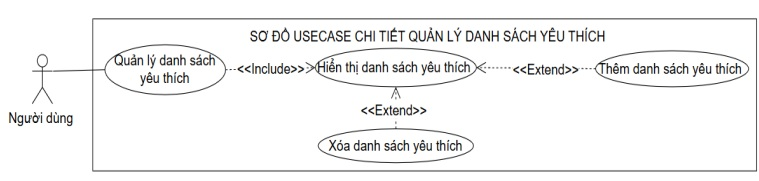
\includegraphics[width=\textwidth]{Chapter_2/Images_c2/usecase.jpg}
    \caption{Sơ đồ use case quản lý danh sách yêu thích} 
    \label{fig-usqlds}
\end{figure}

%-- Nếu có bảng ---
\begin{table}[H]
\centering
\caption{Kết quả thực nghiệm.}
\begin{tabular}{ccccc}
\toprule
\textbf{STT} & \textbf{Model}   & \textbf{Cột A} & \textbf{Cột B} & \textbf{Cột C} \\ 
\midrule
1 & Thuật toán 1        & 1  & 2  & 3            \\
2 & Thuật toán 2       & 4  & 5  & 6            \\
\bottomrule
\end{tabular}
\label{tab-kq}
\end{table}

\subsection{Phân tích 2}

\subsection{Phân tích 3}

\section{KHẢO SÁT - XỬ LÝ SỐ LIỆU MÔ HÌNH, QUY TRÌNH, CÔNG CỤ SỬ DỤNG}

\subsection{KHẢO SÁT - XỬ LÝ SỐ LIỆU MÔ HÌNH}
\subsection{QUY TRÌNH}
\subsection{CÔNG CỤ SỬ DỤNG}

\newpage

\chapter{KẾT QUẢ VÀ THẢO LUẬN}\label{chap3_intro}
\vspace{-40pt}

 
\section{SẢN PHẨM/KẾT QUẢ ĐẠT ĐƯỢC}
\subsection{Kết quả 1}
Nội dung văn bản 

Nội dung đoạn 1


Nội dung đoạn 2 nếu có

\subsection{Kết quả 2}


\subsection{Kết quả 3}


\section{THẢO LUẬN}

\subsection{Đánh giá mức độ đạt mục tiêu đề ra}
Nội dung văn bản
%-- Nếu có hình ---
\begin{figure}[htbp]
    \centering % Bỏ dấu gạch dưới ở đây
    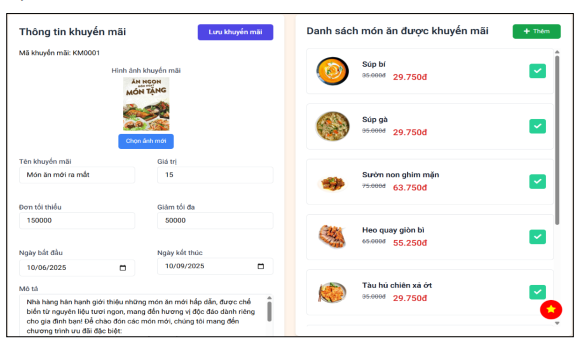
\includegraphics[width=\textwidth]{Chapter_3/Images_c3/khuyenmai.png}
    \caption{Cập nhật chương trình khuyến mãi} 
    \label{fig-logo3}
\end{figure}

%-- Nếu có bảng ---
\begin{table}[H]
\centering
\caption{Kết quả thực nghiệm.}
\begin{tabular}{ccccc}
\toprule
\textbf{STT} & \textbf{Model}   & \textbf{Cột A} & \textbf{Cột B} & \textbf{Cột C} \\ 
\midrule
1 & Thuật toán 1        & 1  & 2  & 3            \\
2 & Thuật toán 2       & 4  & 5  & 6            \\
\bottomrule
\end{tabular}
\label{tab-vidu3}
\end{table}

\subsection{Ưu điểm}

\subsection{Nhược điểm}

\newpage

\chapter{KẾT LUẬN VÀ ĐỀ XUẤT}\label{chap4_intro}
\vspace{-40pt}

\section{KẾT LUẬN}
\begin{itemize}
    \item Kết luận thứ 1: Hệ thống đã hoàn thành việc nghiên cứu và ứng dụng mô hình học máy Random Forest vào bài toán quản lý nhà hàng F\&B đạt kết quả tốt.
    \item Kết luận thứ 2: Xây dựng thành công ứng dụng web có giao diện trực quan, hỗ trợ quản lý bộ phận kho và đặt món trực tuyến.
    \item Kết luận thứ 3: Tối ưu hóa chuỗi cung ứng vật liệu giúp giảm thiểu chi phí vận hành từ 10\% đến 15\%.
\end{itemize}

\section{KIẾN NGHỊ}
\begin{itemize}
    \item Kiến nghị 1: Tiếp tục phát triển mở rộng hệ thống ứng dụng trên nền tảng di động Android và iOS.
    \item Kiến nghị 2: Thử nghiệm tích hợp thêm các thuật toán học sâu nâng cao để dự báo chuỗi thời gian chính xác hơn.
    \item Kiến nghị 3: Mở rộng quy mô áp dụng thực nghiệm tại nhiều chuỗi nhà hàng lớn trên địa bàn.
\end{itemize}
tài liệu: 1 \cite{tapchi} 2 \cite{chuong} 3 \cite{giaotrinh} 4 \cite{luanvan} 5 \cite{hoithao} 6 \cite{internet} 
xin chào: \ac{cnn}

%tài liệu: \cite{tapchi} \cite{chuong} \cite{giaotrinh} \cite{luanvan} %\cite{hoithao} \cite{internet}
% -------------------TÀI LIỆU THAM KHẢO -----------------
% % --- BỌC KHỐI ĐỂ ĐỊNH DẠNG CỠ CHỮ AN TOÀN ---
% \begingroup
%   \fontsize{13}{16}\selectfont   % Định dạng cỡ chữ 13pt, dòng 16pt cho riêng phần này
%   \vspace*{-40pt}                % Đẩy tiêu đề dịch lên trên 40pt một cách độc lập

%   % Gọi lệnh in với tiêu đề thuần túy (Không chèn lệnh font vào đây nữa)
% % %\printbibliography[title={TÀI LIỆU THAM KHẢO}]
% \endgroup
% \newpage
% ------------------- TÀI LIỆU THAM KHẢO -----------------
\newpage
\addcontentsline{toc}{chapter}{TÀI LIỆU THAM KHẢO}

{\centering\bfseries\fontsize{14pt}{18pt}\selectfont TÀI LIỆU THAM KHẢO\par}
\vspace{30pt}

\begingroup
\fontsize{13pt}{16pt}\selectfont
\printbibliography[heading=none]
\endgroup
\newpage
%------------------- PHẦN PHỤ LỤC ĐÍNH KÈM -----------------------
\renewcommand{\thepage}{A-\arabic{page}}
\setcounter{page}{1}
\pagenumbering{roman}
\addtocontents{toc}{\protect\setcounter{tocdepth}{0}}
\chapter*{phụ lục}\label{phuluc_intro}
\vspace{-40pt}
% --- THIẾT LẬP ĐÁNH SỐ HÌNH CHO PHỤ LỤC ---
\setcounter{figure}{0}          % Bắt đầu đếm lại từ số 0
\renewcommand{\thefigure}{\arabic{figure}} % Chỉ hiển thị số thứ tự (Hình 1)
% ------------------------------------------
\renewcommand{\thesection}{\arabic{section}} % Loại bỏ số chương (0) phía trước, chỉ hiện số thứ tự section
% Reset bộ đếm section về 0 để section tiếp theo là số 1
\setcounter{section}{0}
\section{Bổ sung 1}
\begin{figure}[htbp]
    \centering % Bỏ dấu gạch dưới ở đây
    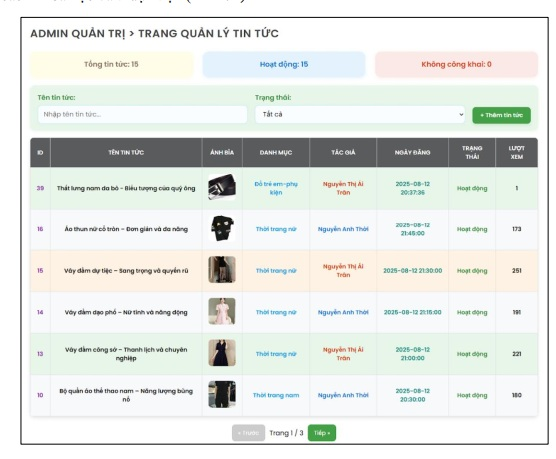
\includegraphics[width=0.7\textwidth]{Appendix/Images_phuluc/giaodientrangquanlytintuc.jpg}
    \caption[]{Giao diện trang quản lý tin tức} 
   
\end{figure}
\clearpage
\section{Bổ sung 2}
\begin{figure}[htbp] % Dùng !t để ép lên đầu trang
    \centering
    
\includegraphics[width=0.7\textwidth]{Appendix/Images_phuluc/chungnhan.jpg}
    \caption[]{Chứng nhận tri thức khoa học trẻ} 
\end{figure}

\clearpage
\section{Bổ sung 3}
\begin{figure}[htbp]
    \centering % Bỏ dấu gạch dưới ở đây
    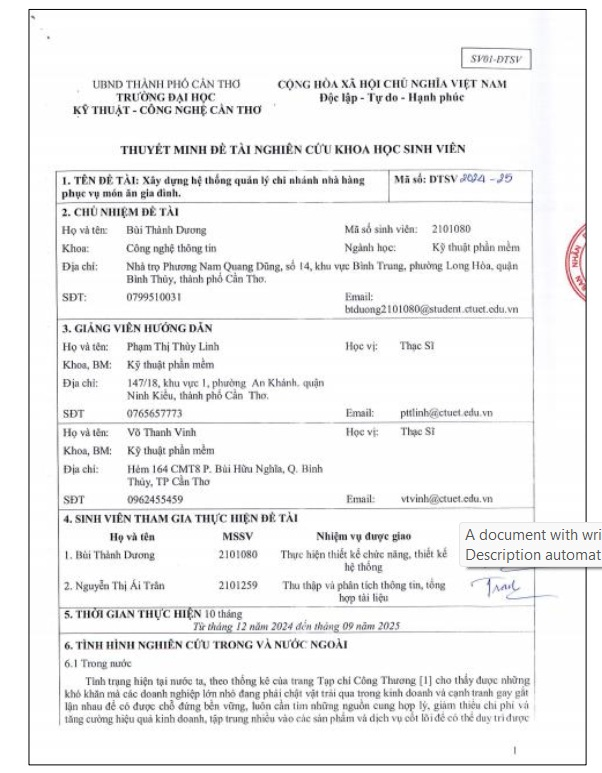
\includegraphics[width=0.7\textwidth]{Appendix/Images_phuluc/nckh.jpg}
    \caption[]{Chứng nhận nghiên cứu khoa học} 
   
\end{figure}
\clearpage


\end{document}